\subsection{Free-Form Visualization}
%A visualization has been provided that emphasizes an important quality about the project with thorough discussion. Visual cues are clearly defined.
Some data are miss-classified in this task. I'll look into which label is the poorest result and I'll put some of the images which are miss-classified.

The distribution of the correctly classified images are Fig.15

\begin{figure}[H]

	\begin{center}
	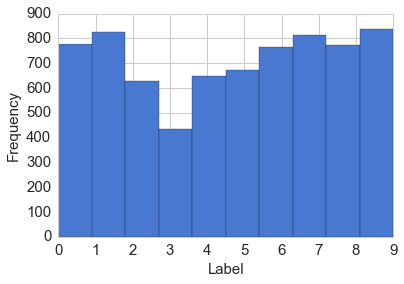
\includegraphics[width=5cm]{picture/label_correct.png}
	\caption{Distribution of the correct prediction}
	\end{center}
	\label{fig:15}

\end{figure}

As you can see, the number of label 3 which is "cat" is apparently small.That means "cat" is overly miss-classified in this dataset.

The Fig.16 shows the distribution of the predicted output. The label 4("deer") and 8("ship") are conspicuously higher than the others. This shows that some of the label are miss classified.

\begin{figure}[H]

	\begin{center}
	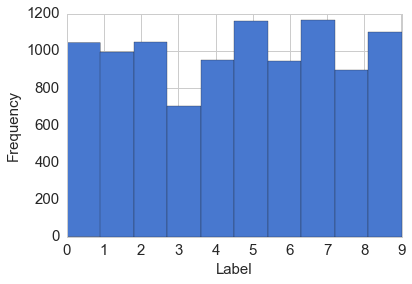
\includegraphics[width=5cm]{picture/output.png}
	\caption{Distribution of the predicted label}
	\end{center}
	\label{fig:16}

\end{figure}





The heatmap below clearly explains the miss-classified data. Label 3("cat") is miss-classified as label 5("dog"). Label 2("bird") and label 7("horse") are miss-classified as label 4("deer"). Label 1("automobile") is miss-classified as label 8("ship").Judging from the heatmap, the miss-classified data are somewhat understandable since some cats are similar to dogs and some automobiles may be similar to ship because of the color and shape(Low resolution may be another reason).




\begin{figure}[H]

	\begin{center}
	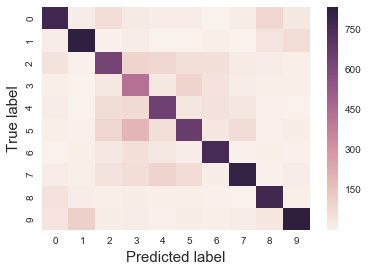
\includegraphics[width=5cm]{picture/heatmap.png}
	\caption{Heatmap of the data}
	\end{center}
	\label{fig:17}

\end{figure}